%----------------------------------------------------------------------------------------
%	Capítulo 1
%----------------------------------------------------------------------------------------


\doublespacing
%% NUEVO CAPITULO X
\chapter{Marco problemático}
%% NUEVA SECCIÓN X.X
\section{Definición de la problemática}

Actualmente, la crianza de o cultivo de truchas en el Perú se da de manera artesanal, los procesos involucrados son realizados por operarios de forma manual. La automatización de procesos manuales aumenta diversos factores que van desde la calidad del producto hasta la capacidad de producción. Una \textbf{empresa nacional} en la \textbf{región de Lima} que se dedica a la producción y venta de trucha arcoíris de diversos gramajes para el mercado nacional, luego de realizar una \textbf{consultoría privada}, detectó altos porcentajes de mortandad y desaparición (cerca del 20\% que representan aproximadamente 18 000 truchas) en la etapa de engorde (17.5 centímetros en adelante).\\

Según la consultoría, \textbf{la mortandad y desaparición de las truchas en la etapa de engorde} se debe a la alta densidad de peces en las jaulas. Las principales causas de un alto grado de desaparición están asociadas a la característica carnívora de las truchas, es decir, pueden alimentarse de otras truchas. Las truchas deben ser clasificadas periódicamente en sus respectivas jaulas flotantes, según tamaño. Sin embargo, debido a la complejidad y cantidad de esfuerzo requerido, (3 operarios para una jaula de 3 metros cúbicos que contienen 5000 truchas requieren 40  horas de trabajo) la clasificación no es muy frecuente. Además, realizar el proceso de forma manual incide en el comportamiento de la trucha, pudiendo causar una muerte por estrés. Debido a esto, \textbf{el presente trabajo busca automatizar dicho proceso}.\\

%% NUEVO SUBSECCION X.X.X
\subsection{Justificación}

Según la empresa nacional, reducir la mortandad en el cultivo artesanal de truchas aumentará la capacidad de producción. Se detalla que cuando dichas truchas atraviesan las etapas de \textit{alevinos III} (7.5 a 10.0 cm.), \textit{juvenil I} (10.0 a 13.5 cm.) y \textit{engorde} (17 cm. en adelante) aumenta la mortandad considerablemente, siendo los dos últimos los más importantes. La mortandad de truchas se da por diversos motivos, entre ellos, el más importante, la falta de clasificación correcta de truchas según su tamaño.\\

La clasificación y conteo realizado por operarios de forma manual requiere excesivo tiempo y mano de obra. Esto puede agravarse ya que en tiempos de mayor presencia fluvial se realiza el trabajo bajo condiciones meteorológicas adversas que dificultan el trabajo haciéndolo más lento y en oportunidades inviable debido a que se requiere el uso de generadores de electricidad, hacer uso de estos en esas condiciones puede generar accidentes. \\

%% NUEVO SUBSECCION X.X.X
\subsection{Alcance}
Este trabajo busca diseñar un sistema clasificador y contador de truchas arcoíris de un determinado rango de tamaños. De igual forma, se busca integrar nuevas tecnologías y métodos, según sean viables bajo el análisis del diseño conceptual y preliminar del sistema mecatrónico, a los sistemas. Además, se busca integrar los sistemas de clasificación y conteo de truchas.
La cuantificación de producción brindará una idea clara de los beneficios que puede aportar un sistema mecatrónico al cultivo de truchas arcoíris en lagunas. \\

%% NUEVO SUBSECCION X.X.X
\subsection{Objetivos}

%% NUEVA SUB-SUB-SECCION X.X.X.X
\subsubsection{Objetivo general}

Diseñar un sistema clasificador y contador truchas arcoíris de 10 a 20 centímetros.

%% NUEVA SUB-SUB-SECCION X.X.X.X
\subsubsection{Objetivos específicos}

\begin{itemize}
\item Identificar procesos críticos en la crianza artesanal de trucha arcoíris.
\item Diseñar un sistema de clasificación.
\item Diseñar un sistema de conteo de truchas.
\item Cuantificar la capacidad de producción del sistema de recepción, clasificación y conteo de truchas arcoíris.
\end{itemize}

%% NUEVO SUBSECCION X.X.X
\subsection{Metodología}

La metodología, que contempla las recomendaciones para encontrar una solución óptima, está basada en el libro \textit{Engineering Design – A Systematic Approach}.\footnote{Traducción: \textit{"Diseño de ingeniería: un enfoque sistemático"}}  Esta metodología puede incluir múltiples normas de diseño, en este caso las normas VDI 2221-2225 \textit{(La Asociación de Ingenieros Alemanes)}.  \\

El análisis, el términos generales, consiste en recopilar información, realizar una lista de requerimientos, discernir entre procesos críticos que pueden ser automatizados, separar los procesos en sistemas que cumplan funciones, listar las mejores opciones para cada subsistema, iterar hasta encontrar la solución más óptima que integre todos los subsistemas, proponer tres o más soluciones óptimas como concepto de solución, seleccionar una de estas, seleccionar materiales y procesos de fabricación, seleccionar componentes comerciales para cada dispositivo elegido para el concepto de solución, realizar cálculos de diseño, realizar planos de diseño y presentar una propuesta final. En cada etapa del diseño la parte conceptual puede variar, pero los principios de funcionamiento deben prevalecer.\\

%% NUEVA SECCIÓN X.X
\section{Estado del arte}
\textbf{El estado del arte es una categoría central y deductiva que se aborda y propone como estrategia un análisis crítico} de las dimensiones políticas, epistemológicas y pedagógicas de la producción investigativa en la evaluación de aprendizaje.\cite{GuevaraPatino2016} \textbf{El aspecto técnico del estado del arte, al que se hace referencia en este estudio, se basa en el desarrollo de una investigación técnica documental y técnica de campo.} La técnica documental permite la selección de información para explicar las teorías que sustentan el estudio de los fenómenos y procesos.. \cite{Martinez2003} Además, las técnicas de investigación de campo son aquellas que el investigador utiliza en el desarrollo práctico o teórico de su proceso investigativo con el fin de corroborar sus objetivos generales y específicos. \cite{GuevaraPatino2016}\\

Luego de mencionar el enfoque de este subíndice, \textbf{aclarar} que, en términos técnicos, existe una diferencia clara entre clasificación de peces y pescado. Esta diferencia se basa en que el pez se refiere al animal vivo y el pescado es el animal muerto. \\

%% NUEVO SUBSECCION X.X.X
\subsection{Crianza de truchas}

%% NUEVA SUB-SUB-SECCION X.X.X.X
\subsubsection{Nacional}
En el Perú, el \textbf{cultivo de trucha se da predominantemente de forma manual} ya que el sector es dirigido por pequeñas y medianas empresas. La capacidad de producción del Perú es alta debido a la gran cantidad de especies, recursos hidrobiológicos\footnote{Se refieren a los organismos que pasan toda su vida o parte de ella en un ambiente acuático y son utilizados por el hombre de forma directa o indirecta.\cite{MINAGRI2011}} y climas. \\

\textbf{El gobierno peruano implementó medidas} para impulsar su desarrollo mediante el MEF\footnote{Ministerio de Economía y Finanzas.}  en el marco de estrategia de Gobierno de impulsar y promocionar los sectores con alto potencial productivo. \textbf{Las medidas acuícolas se centran en seis ejes}: primero, fortalecimiento de la Autoridad Sanitaria; segundo, una regulación que garantice el cumplimiento de estándares de sanidad, inocuidad, ambientales y de calidad de los productos; tercero, escalar y abrir nuevos mercados para las exportaciones acuícolas; cuarto, impulsar la gestión y articulación interinstitucional; quinto, promocionar apoyo tecnológico e innovación en especial para las micro y pequeñas empresas; sexto, mejorar infraestructura. \cite{Andina2019}\\

\begin{figure}[H]
	\centering
	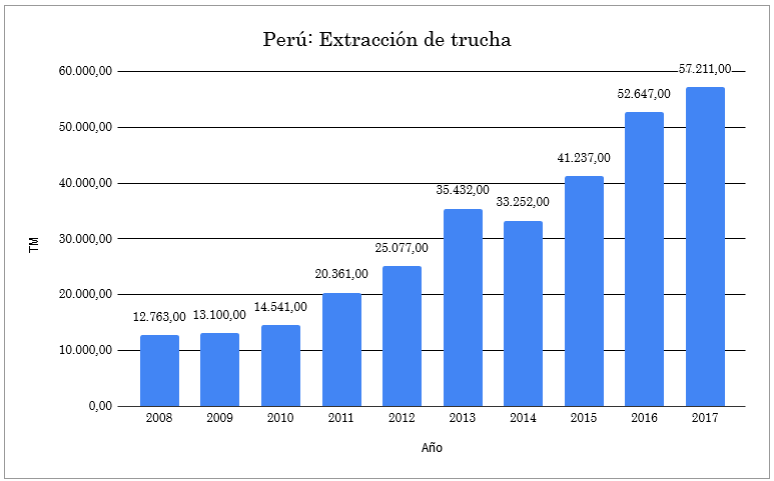
\includegraphics[width=1\textwidth]{chapter1/extraccion trucha toneladas anuales.png}
	\caption{Extracción de trucha en toneladas métricas anuales.}
	 Datos \cite{MinisteriodelaProducciondelPeru2018}\\
	  Gráfica: Elaboración propia.
	\label{fig:Extracción de trucha en toneladas métricas anuales}
\end{figure}

%% NUEVA SUB-SUB-SECCION X.X.X.X
\subsubsection{Internacional}

En \textbf{China}\footnote{Asia concentra alrededor del 90\% de la acuicultura mundial.\cite{Powell2003}}, principal país exportador en acuicultura a nivel mundial con 20 mil millones de dólares \cite[p.~44]{FAO2017}, se usa métodos de crianza de truchas que reducen la \textit{mortandad} y el \textit{estrés hídrico} que afectan a las truchas. Procesos automatizados y estandarizados aumentaron la producción de trucha arcoíris a nivel internacional. Lograron una reducción importante de costos en el cultivo debido a la automatización. Se controla la calidad de agua, contaminación por exceso de excremento de las truchas, temperatura del agua, tasa de crecimiento, etc. \cite[p.~1-6]{2017} \\

En \textbf{Japón}, segundo país que más importa productos pesqueros a nivel mundial \cite[p.~44]{FAO2017}, produce alrededor de 50000 especies de peces, lo que representa aproximadamente 10 mil toneladas anuales. La crianza de truchas se da en estanques de agua corriente, en lagunas y en aguas marinas profundas (estanques con agua de mar bombeadas desde la profundidad del océano 100 m. o más). Sin embargo, nuevas invasiones de patógenos están mermando la producción y debido a esto se crearon fármacos. La industria se encuentra altamente industrializada. \cite[p.~1-5]{2005} \\

En el \textbf{\ref{Productos comerciales y patentes}} se muestran productos y patentes de origen internacional, desarrollados para el sector acuícola y que son cercanos al estudio en este trabajo.

\begin{table}[H]
	\centering	
	\caption{Comercio internacional de productos pesqueros por principales importadores y exportadores en miles de dólares.}
	\label{tbl:comercio internacional de productos pesqueros por principales importadores y exportadores en dolares}
	\begin{tabular}{ | c | }
		\hline
		\begin{minipage}{1\textwidth}
			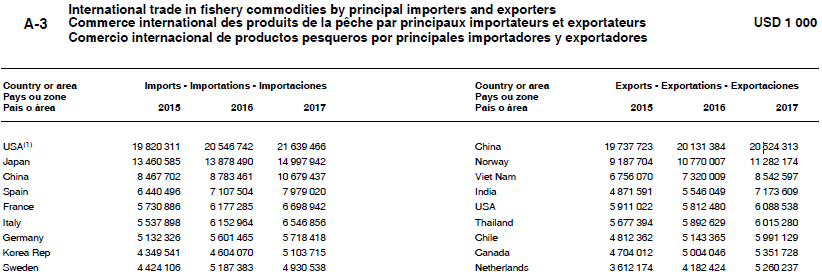
\includegraphics[width=1\textwidth]{chapter1/comercio internacional de productos pesqueros por principales importadores y exportadores en dolares.png}
		\end{minipage}		
		\\ \hline
	\end{tabular}
	\\	Fuente: FAO.
\end{table}

%% NUEVO SUBSECCION X.X.X
\subsection{Sistema de clasificación de peces}
Existen \textbf{dos dimensiones} en las que se basa la clasificación: \textbf{la distancia desde la boca hasta la aleta caudal} en sus respectivos extremos y \textbf{la circunferencia} que alrededor del pez cerca del inicio de la aleta dorsal. En la Figura \ref{fig:anatomia de la trucha arcoiris} se muestra la anatomía de la especie y se puede observar las regiones de la trucha. \\

En la práctica, sabiendo que se puede aproximar una medida a partir de la otra, so-lo se toma la distancia que cubre las tres regiones.\footnote{La toma de datos de manera manual suele ser hasta 100 veces más lenta que otros métodos.} \\

Se realiza este proceso para evitar problemas que afecten negativamente la producción: truchas en competencia por alimento, aumento de diferencia en tallas, reducción del rendimiento del alimento, aumento de mortandad en los peces de menor talla, disminución de calidad y talla. Con una clasificación adecuada y oportuna se trata de \textbf{prevenir el canibalismo}\footnote{Las truchas son carnívoras por lo que pueden alimentarse de su misma especie, en este caso de los de menor talla.}, uniformizar el crecimiento para brindar una alimentación adecuada a la talla, prevenir estrés y agotamiento de los peces.\cite[p.~16]{Flores2010} \\

\begin{figure}[H]
	\centering
	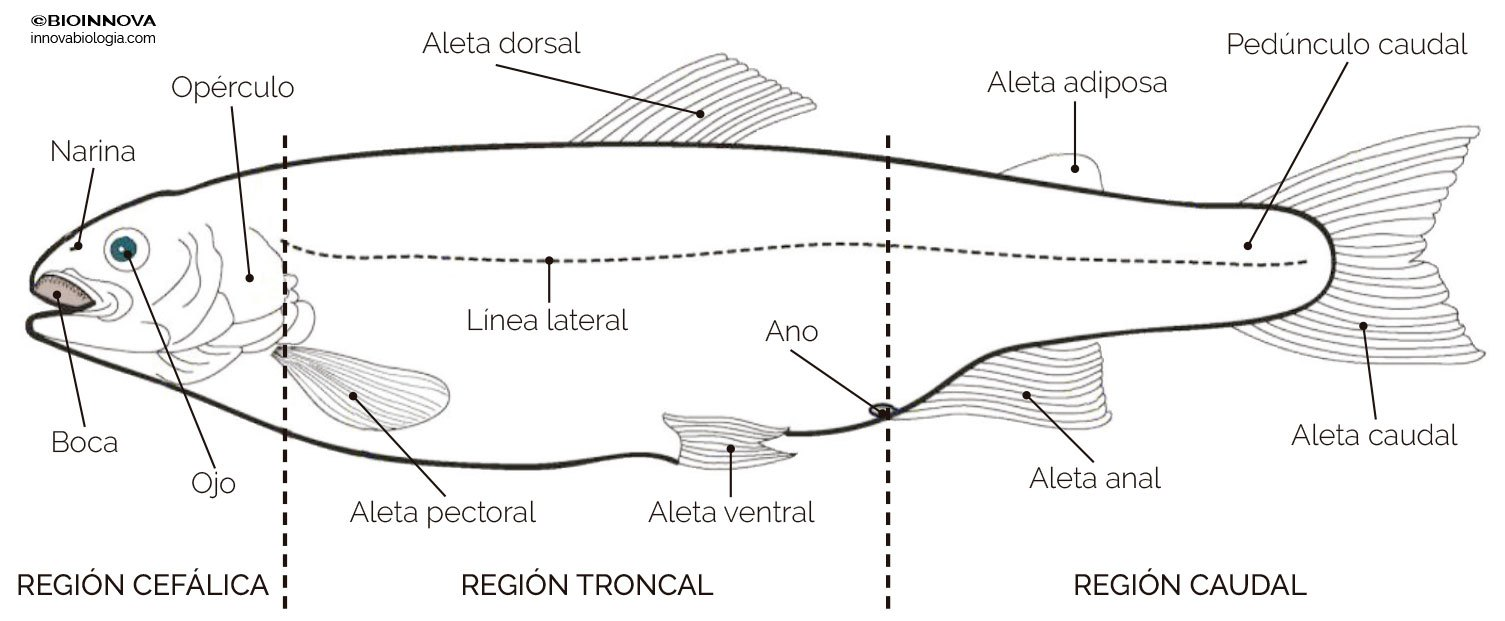
\includegraphics[width=1\textwidth]{chapter1/anatomia de la trucha arcoiris.png}
	\caption{Anatomía de la trucha arcoíris \textit{(Oncorhynchus mykiss)}.}
	Fuente: Bioinnova.
	\label{fig:anatomia de la trucha arcoiris}
\end{figure}


La clasificación por tamaño permite identificar en qué etapa de producción se encuentra la trucha. Identificar las etapas permite brindar un plan de alimentación adecuado y reducir la sobre-alimentación. En la Tabla \ref{tbl:clasificacion de truchas por etapas de produccion} se muestra las etapas existentes según FONDEPES\footnote{Fondo Nacional de Desarrollo Pesquero}.


% Please add the following required packages to your document preamble:
% \usepackage[table,xcdraw]{xcolor}
% If you use beamer only pass "xcolor=table" option, i.e. \documentclass[xcolor=table]{beamer}
\begin{table}[]
	\centering	
	\caption{Clasificación de truchas por etapas de producción.}
	\label{tbl:clasificacion de truchas por etapas de produccion}
	\begin{tabular}{l|c|c|c|c|c|c|c|c|c|}
		\cline{2-10}
		& \cellcolor[HTML]{9B9B9B}{\color[HTML]{000000} \textbf{\rot{Siembra}}} & \cellcolor[HTML]{9B9B9B}{\color[HTML]{000000} \textbf{\rot{Alevinaje I}}} & \cellcolor[HTML]{9B9B9B}{\color[HTML]{000000} \textbf{\rot{Alevinaje II}}} & \cellcolor[HTML]{9B9B9B}{\color[HTML]{000000} \textbf{\rot{Alevinaje III}}} & \cellcolor[HTML]{9B9B9B}{\color[HTML]{000000} \textbf{\rot{Juvenil I}}} & \cellcolor[HTML]{9B9B9B}{\color[HTML]{000000} \textbf{\rot{Juvenil II}}} & \cellcolor[HTML]{9B9B9B}{\color[HTML]{000000} \textbf{\rot{Engorde I}}} & \cellcolor[HTML]{9B9B9B}{\color[HTML]{000000} \textbf{\rot{Engorde II}}} & \cellcolor[HTML]{9B9B9B}{\color[HTML]{000000} \textbf{\rot{Cosecha}}} \\ \hline
		\multicolumn{1}{|l|}{\cellcolor[HTML]{9B9B9B}\textbf{De \textit{(mm)}}} & - & 35 & 51 & 81 & 121 & 141 & 171 & 201 & 261 \\ \hline
		\multicolumn{1}{|l|}{\cellcolor[HTML]{9B9B9B}\textbf{Hasta \textit{(mm)}}} & 34 & 50 & 80 & 120 & 140 & 170 & 200 & 260 & - \\ \hline
		\multicolumn{1}{|l|}{\cellcolor[HTML]{9B9B9B}\textbf{De \textit{(g)}}} & - & 2.81 & 6.91 & 11 & 51 & 110 & 153 & 200 & 251 \\ \hline
		\multicolumn{1}{|l|}{\cellcolor[HTML]{9B9B9B}\textbf{Hasta \textit{(g)}}} & 2.80 & 6.90 & 10 & 50 & 109 & 152 & 199 & 250 & 290 \\ \hline
		\multicolumn{1}{|l|}{\cellcolor[HTML]{9B9B9B}\textbf{Este trabajo \textit{(mm)}}} & \multicolumn{3}{c|}{} & \multicolumn{4}{c|}{\cellcolor[HTML]{C0C0C0}100 a 200} & \multicolumn{2}{c|}{} 
		\\ \hline
	\end{tabular}
	\\Fuente: FONDEPES.
\end{table}

%% NUEVA SUB-SUB-SECCION X.X.X.X
\subsubsection{Clasificación manual}

La clasificación manual se \textbf{recomienda cuando la cantidad de truchas no supera las 1000 truchas}.\cite[p.~25]{FAO2014} Las cajas clasificadoras ya sean de anchura fija o ajustables son fabricadas artesanalmente como las mostradas en la Figura \ref{fig:clasificadora de anchura fija rejillas de clasificacion y clasificadora ajustable} Estas cajas de madera y metal con barras de metal o compuestos montados en su base dejan pasar por las rejillas a los peces que tienen determinada circunferencia, es decir, se realiza una clasificación por forma.\cite{FAO2005} \\

\begin{figure}[H]
	\centering
	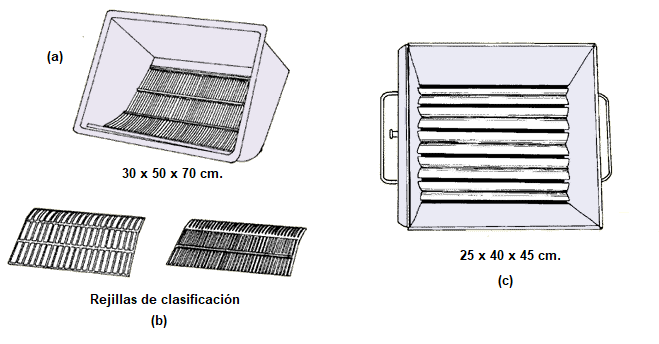
\includegraphics[width=1\textwidth]{chapter1/clasificadora de anchura fija rejillas de clasificacion y clasificadora ajustable.png}
	\caption{(a,b,c) Clasificadora de anchura fija, rejillas de clasificación y clasificadora ajustable.}
	Fuente: FAO.
	\label{fig:clasificadora de anchura fija rejillas de clasificacion y clasificadora ajustable}
\end{figure}

Para realizar el proceso de clasificación manual (Figura \ref{fig:clasificacion y medicion manual de truchas}) se siguen tareas consecutivas: limpiar la caja clasificadora, preparar los estanques o jaulas flotantes que intervienen en la clasificación, ubicar la caja clasificadora al borde del estanque o jaula, extraer con la sacadera telescópica\footnote{Herramienta para trasladar peces. También llamada "\textit{chinguillo}".} truchas de un estanque o jaula, depositar las truchas extraídas dentro de la caja, agitar la caja hasta apreciar que las truchas no pueden pasar y finalmente depositar las truchas restantes en otro estanque o jaula.\\

\begin{figure}[H]
	\centering
	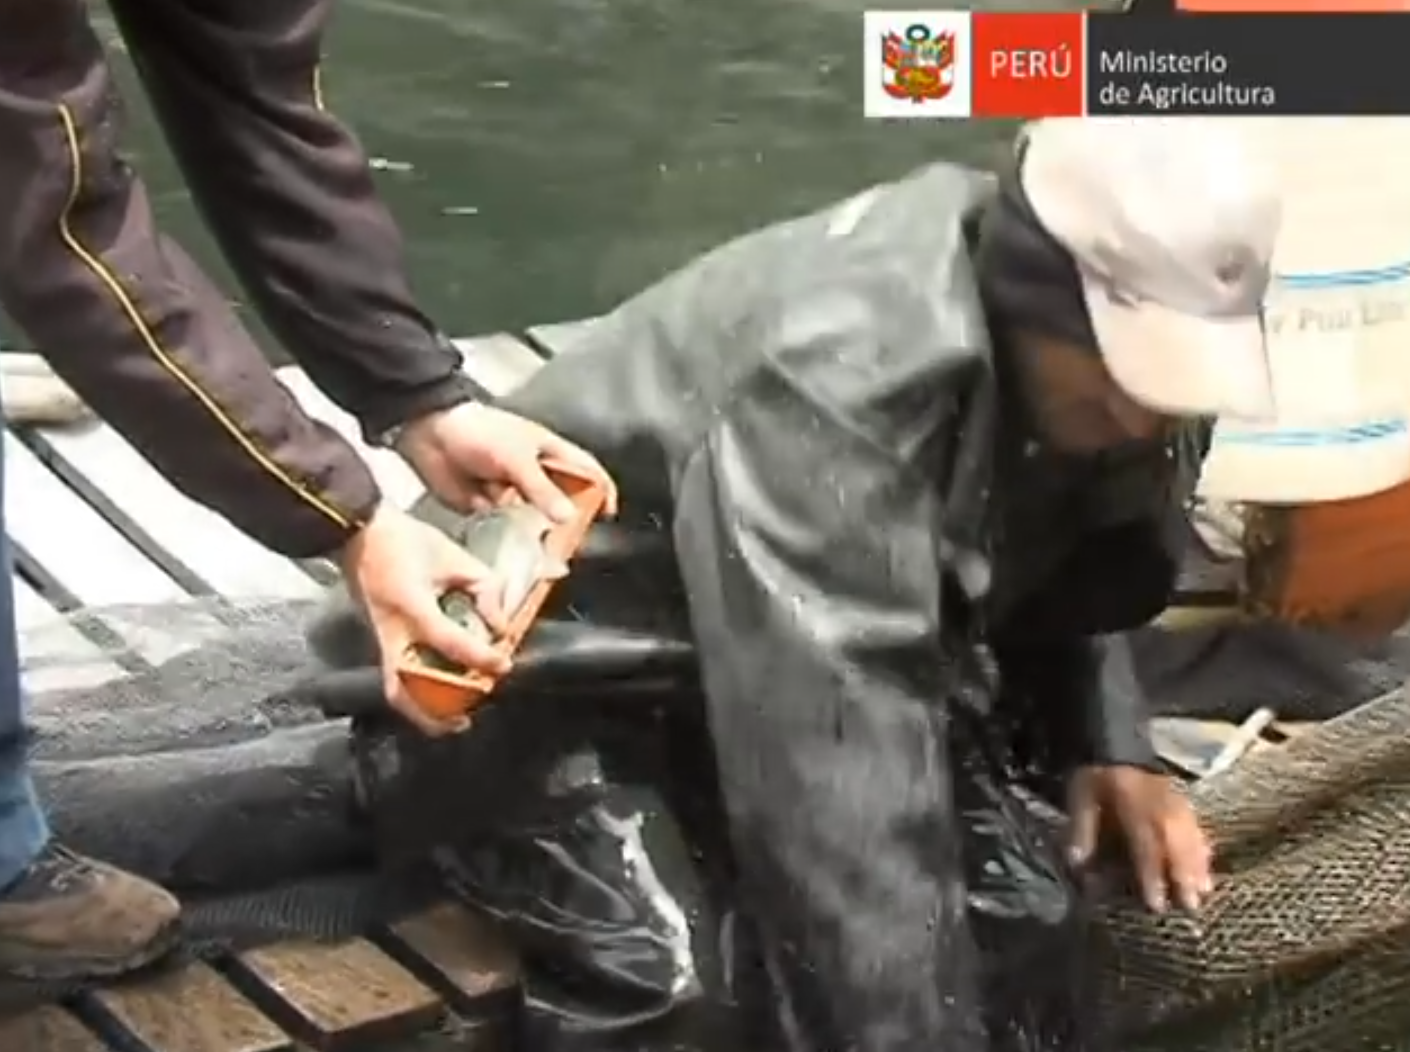
\includegraphics[width=1\textwidth]{chapter1/clasificacion y medicion manual de truchas.png}
	\caption{Clasificación y medición manual de truchas.}
	Fuente: MINAGRI\footnote{Ministerio de Agricultura y Riego del Perú.}.
	\label{fig:clasificacion y medicion manual de truchas}
\end{figure}

Para la medición se usa una herramienta, como la mostrada en la Figura \ref{fig:herramienta de medicion manual para peces},creada \textbf{artesanalmente} que contiene un ictiómetro para medir al pez mientras se realiza una clasificación o verificar el tamaño del pez. \\

\begin{figure}[H]
	\centering
	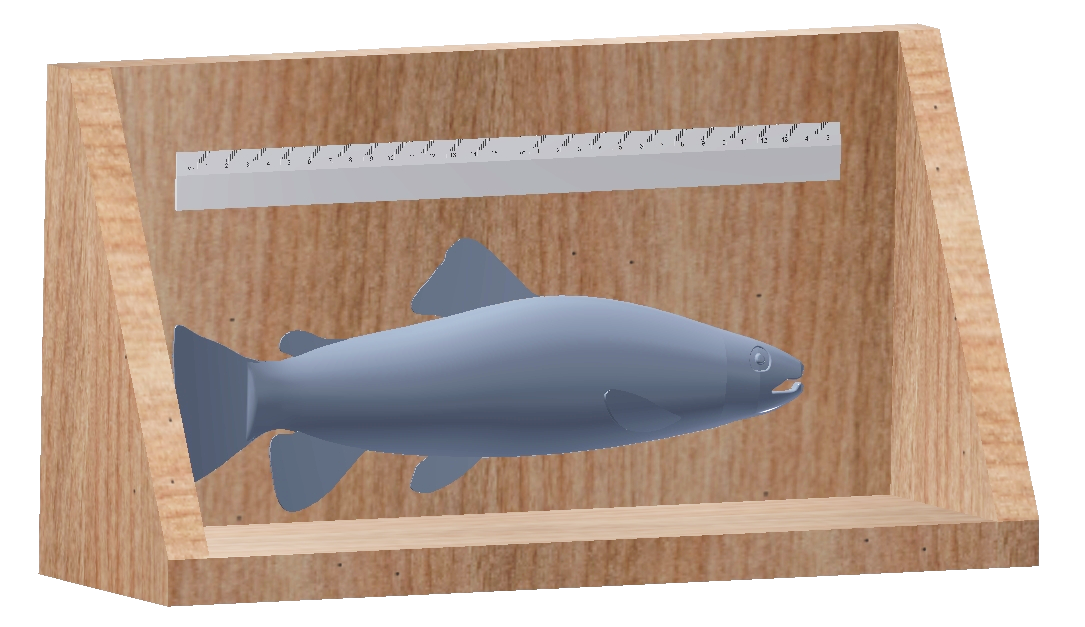
\includegraphics[width=1\textwidth]{chapter1/herramienta de medicion manual para peces.png}
	\caption{Herramienta de medición manual para peces.}
	Fuente: Elaboración propia.
	\label{fig:herramienta de medicion manual para peces}
\end{figure}

%% NUEVA SUB-SUB-SECCION X.X.X.X
\subsubsection{Clasificación mecánica}

La tesis que presentó el bachiller \textit{Angel Gabriel Vega De la Cruz} desarrolla un sistema mecánico que, asegura, permite seleccionar los peces de manera rápida y eficiente. El sistema mecánico consiste en un motor-reductor, un sistema de alimentación compuesto por cuatro poleas y dos bandas transportadoras. La Figura \ref{fig:maquina seleccionadora de truchas agv} nos muestra la máquina, la cual puede clasificar tres rangos de  diferentes capacidades de selección (18000, 7200 y 3600 peces/hora) a un precio estimado de S/ 19264,27 en 2013. Otro factor importante es el peso de la máquina: 200 kg.\cite[p.~2,105]{Vega2013} \\

\begin{figure}[H]
	\centering
	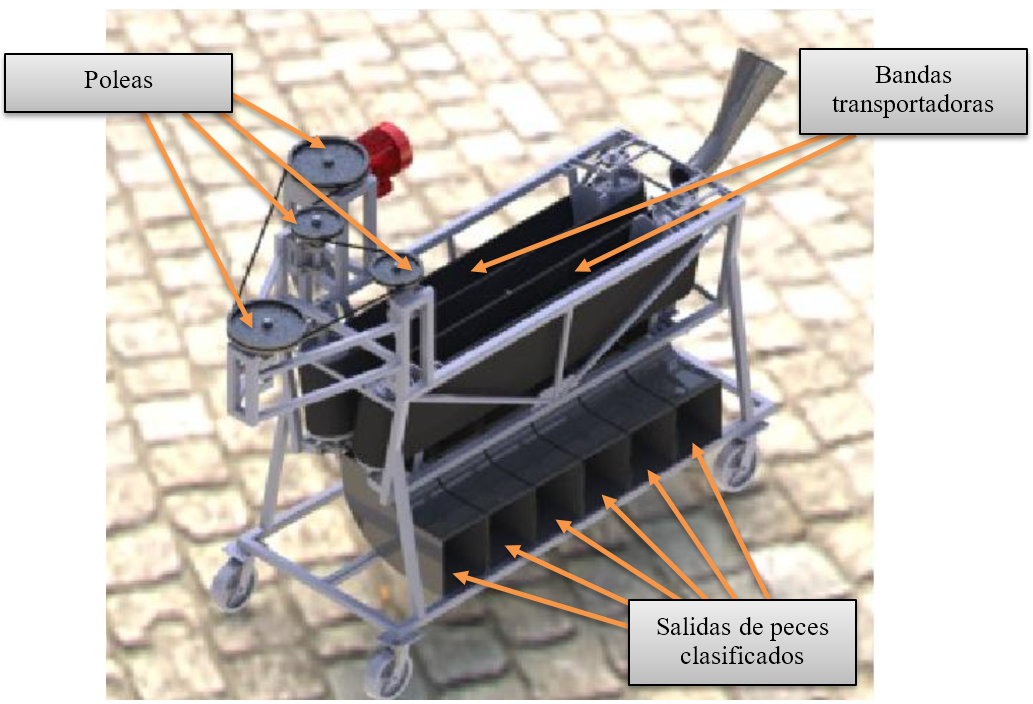
\includegraphics[width=1\textwidth]{chapter1/maquina seleccionadora de truchas agv.png}
	\caption{Máquina seleccionadora de truchas de A. G. V.}
	Fuente: Tesis “Diseño de una Máquina Seleccionadora de Truchas”.
	\label{fig:maquina seleccionadora de truchas agv}
\end{figure}

%% NUEVA SUB-SUB-SECCION X.X.X.X
\subsubsection{Clasificación mediante visión por computadora}

Este tipo de clasificación completamente automatizada permite un conteo de peces más rápido con respecto a otros métodos. Los avances en esta área son abundantes, se presentarán los que aborden los objetivos de este trabajo. La capacidad de conteo depende en dos factores principales. \cite[p.~2-3]{Niu2018}

\begin{figure}[H]
	\centering
	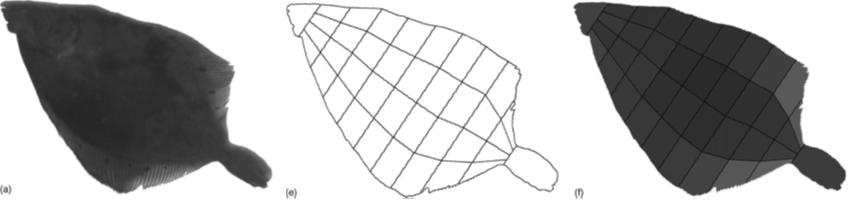
\includegraphics[width=1\textwidth]{chapter1/medicion automatizada de especies y tallas de peces por vision artificial.png}
	\caption{Medición automatizada de especies y tallas de peces por visión artificial.}
	(a,b,c,d,e,f) Imagen original, bordes, 100 puntos de borde, ejes principales y centro con líneas, enmallado, totalmente procesado.\\
	Fuente: \cite[p.~4]{White2006}.
	\label{fig:medicion automatizada de especies y tallas de peces por vision artificial}
\end{figure}

\begin{figure}[H]
	\centering
	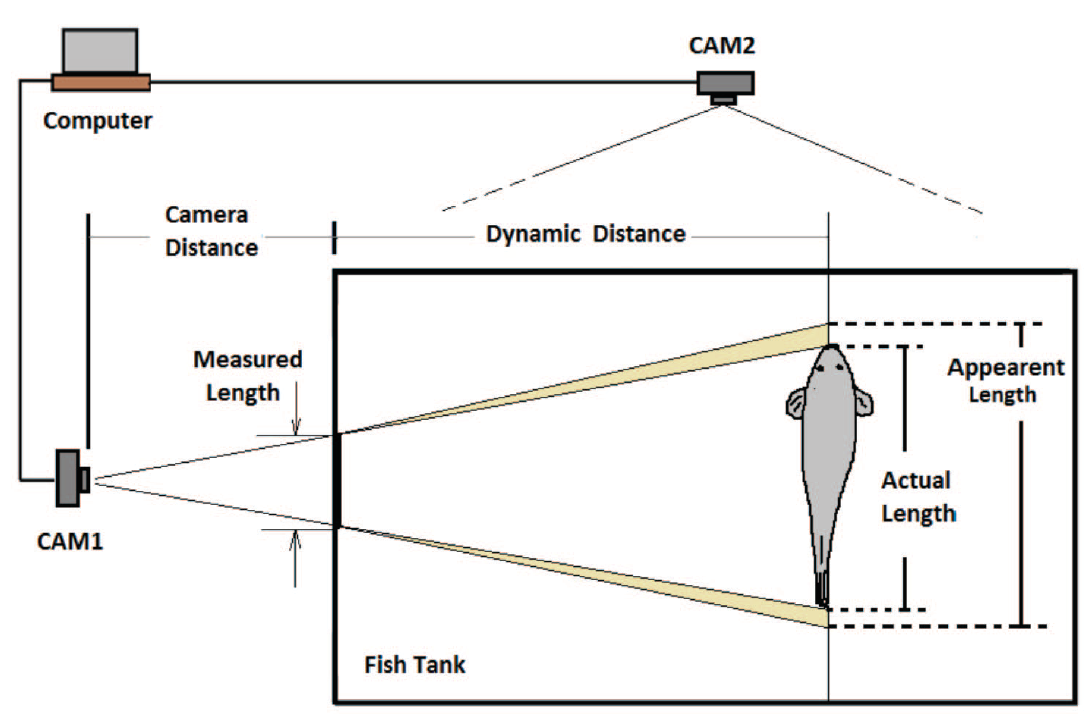
\includegraphics[width=0.75\textwidth]{chapter1/medicion de peces dentro de estanques con camaras ortogonales.png}
	\caption{Medición de  peces dentro de estanques con cámaras ortogonales.}
	Fuente: \cite{Al-Jubouri2017}.
	\label{fig:medicion de peces dentro de estanques con camaras ortogonales}
\end{figure}

\begin{figure}[H]
	\centering
	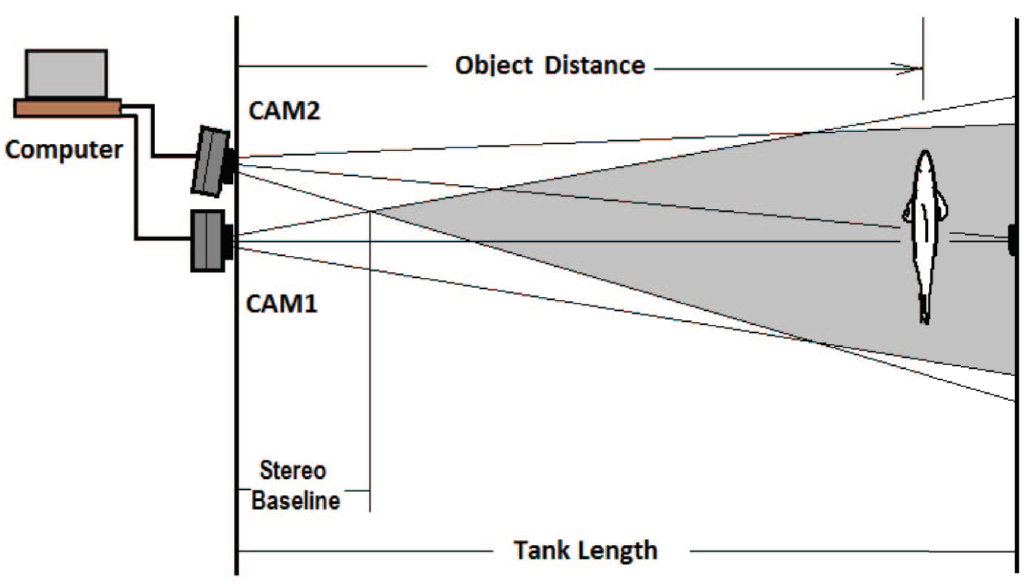
\includegraphics[width=0.75\textwidth]{chapter1/medicion de peces dentro de estanques con camaras estereo.png}
	\caption{Medición de  peces dentro de estanques con cámaras estéreo.}
	Fuente: \cite{Al-Jubouri2017}.
	\label{fig:medicion de peces dentro de estanques con camaras estereo}
\end{figure}

En la Figura \ref{fig:medicion de peces dentro de estanques con camaras ortogonales} y Figura \ref{fig:medicion de peces dentro de estanques con camaras estereo} se muestra dos métodos para extraer la medida real de un pez para poder ser clasificado. El primero muestra un arreglo ortogonal de cámaras, en el caso de poder acceder en dos planos del estanque. El segundo muestra un arreglo que permite medir distancias entre puntos de interés mediante el uso de solo un plano del estanque.

%% NUEVA SUB-SUB-SECCION X.X.X.X
\subsubsection{Clasificación usando técnicas de inteligencia artificial}

Esta tecnología es robusta, es decir, funciona aceptablemente con ruido, cambios en condiciones ambientales, cambios en la adquisición de datos, entre otros cambios. La técnica se basa en redes neuronales , con las que se logra una gran precisión para detectar y segmentar objetos en muchas diferentes condiciones (en este caso peces).
























%% Contenido
%\begin{spacing}{1.5}
%{Ejemplo de cuerpo y ejemplo de imagen en l \ref{fig:PLACEHOLDER}. }
%\begin{equation} \label{eq:1}
%    S=\sum_iP_ilog(P_i)
%\end{equation}
%\end{spacing}
%% Fin de contenido